\documentclass[9pt,twocolumn,twoside]{osajnl}

\journal{ol} % Choose journal (ao, aop, josaa, josab, ol)

% See template introduction for guidance on setting shortarticle option
\setboolean{shortarticle}{true} 
% true = letter / tutorial 
% false = research / review article 
% (depending on journal).

\ifthenelse{\boolean{shortarticle}}{\colorlet{color2}{color2b}}{\colorlet{color2}{color2}} % Automatically switches colors for short articles

\title{Optical Mapping Near-eye 3D Display with Correct Focus Cues}

\author[1,2]{Wei Cui}
\author[1,2,*]{Liang Gao}

\affil[1]{Department of Electrical and Computer Engineering, University of Illinois at Urbana-Champaign, 306 N. Wright St., Urbana, IL 61801, USA}
\affil[2]{Beckman Institute for Advanced Science and Technology, University of Illinois at Urbana-Champaign, 405 N. Mathews Ave., Urbana, IL 61801, USA}

\affil[*]{Corresponding author: gaol@illinois.edu}

\dates{Compiled \today}

\ociscodes{(170.0110) Imaging systems; (330.7322) Visual optics, accommodation; (070.6120) Spatial light modulators.}

\doi{\url{http://dx.doi.org/XX.XXXX/OL.XX.XXXXXX}}

\begin{abstract}
A novel optical mapping method for near-eye 3D displays (OMNI) is developed. Capable of displaying four focal planes for a depth range of 3 diopters with correct focus cues with the application of depth-weighted blending that accommodates the natural stimuli of human eyes, the proposed method can alleviate issues caused by the vergence-accommodation conflict in the conventional stereoscopic displays. The design and implementation of the OMNI display are presented. The experimental results and the performance evaluation of the prototype system are also discussed in detail.
\end{abstract}

\setboolean{displaycopyright}{true}

\begin{document}

\maketitle
\thispagestyle{fancy}

\ifthenelse{\boolean{shortarticle}}{\ifthenelse{\boolean{singlecolumn}}{\abscontentformatted}{\abscontent}}{}

Near-eye three-dimensional (3D) displays have seen rapid growth and held great promise in a variety of applications, such as gaming, film viewing, and professional scene simulations.  Currently, most near-eye 3D displays are based on computer stereoscopy \cite{geng2013three}, which presents two images with parallax in front of the viewer’s eyes. Stimulated by binocular disparity cues, the viewer’s brain then creates an impression of the 3D structure of the portrayed scene. However, the stereoscopic displays suffer from a major drawback—the vergence-accommodation conflict \cite{hoffman2008vergence}—which reduces the viewer’s ability to fuse the binocular stimuli while causing discomfort and fatigue. Because the images are displayed at one surface, the focus cues specify the depth of display screen (\textit{i.e.}, accommodation distance) rather than the depths of depicted scenes (\textit{i.e.}, vergence distance). This is opposite to the viewer’s perception in the real world where these two distances are always the same. To alleviate this problem, one must present correct focus cues that are consistent with binocular disparity cues.

Currently, only a few approaches can provide correct or nearly correct focus cues for the depicted scene, namely light field near-eye displays \cite{hu2014high} and multi-plane near-eye displays \cite{hu2014design}.  The light field display employs a lenslet array to project multi-view images simultaneously onto the viewer’s retina, thereby yielding a continuous 3D sensation. Despite a compact form factor, the spatial resolution is low ($\sim$100×100 pixels \cite{hua20143d}), restricted by the number of pixels that can fit into the imaging area of a lenslet \cite{grzegorzek2013time}. By contrast, the multi-plane display projects two-dimensional (2D) images onto a variety of depth planes through either temporal multiplexing \cite{llull2015design} or spatial multiplexing \cite{reichow2014three}. By synchronizing a fast display with a deformable mirror \cite{hu2014high} or a focal sweeping lens \cite{llull2015design}, the temporal-multiplexing-based methods project depth images in sequence.  However, to render continuous motion, the device must display all depth images within the flicker fusion time (1/60 s), thus introducing a severe trade-off between image dynamic range and the number of depth planes. On the other hand, the spatial-multiplexing-based methods deploy multiple screens at varied distances from the viewer, followed by optically combining their images using a beam splitter. Notwithstanding a high spatial resolution and image dynamic range, the resultant system is bulky and therefore unsuitable for wearable applications.  

\begin{figure}[tbp]
\centering
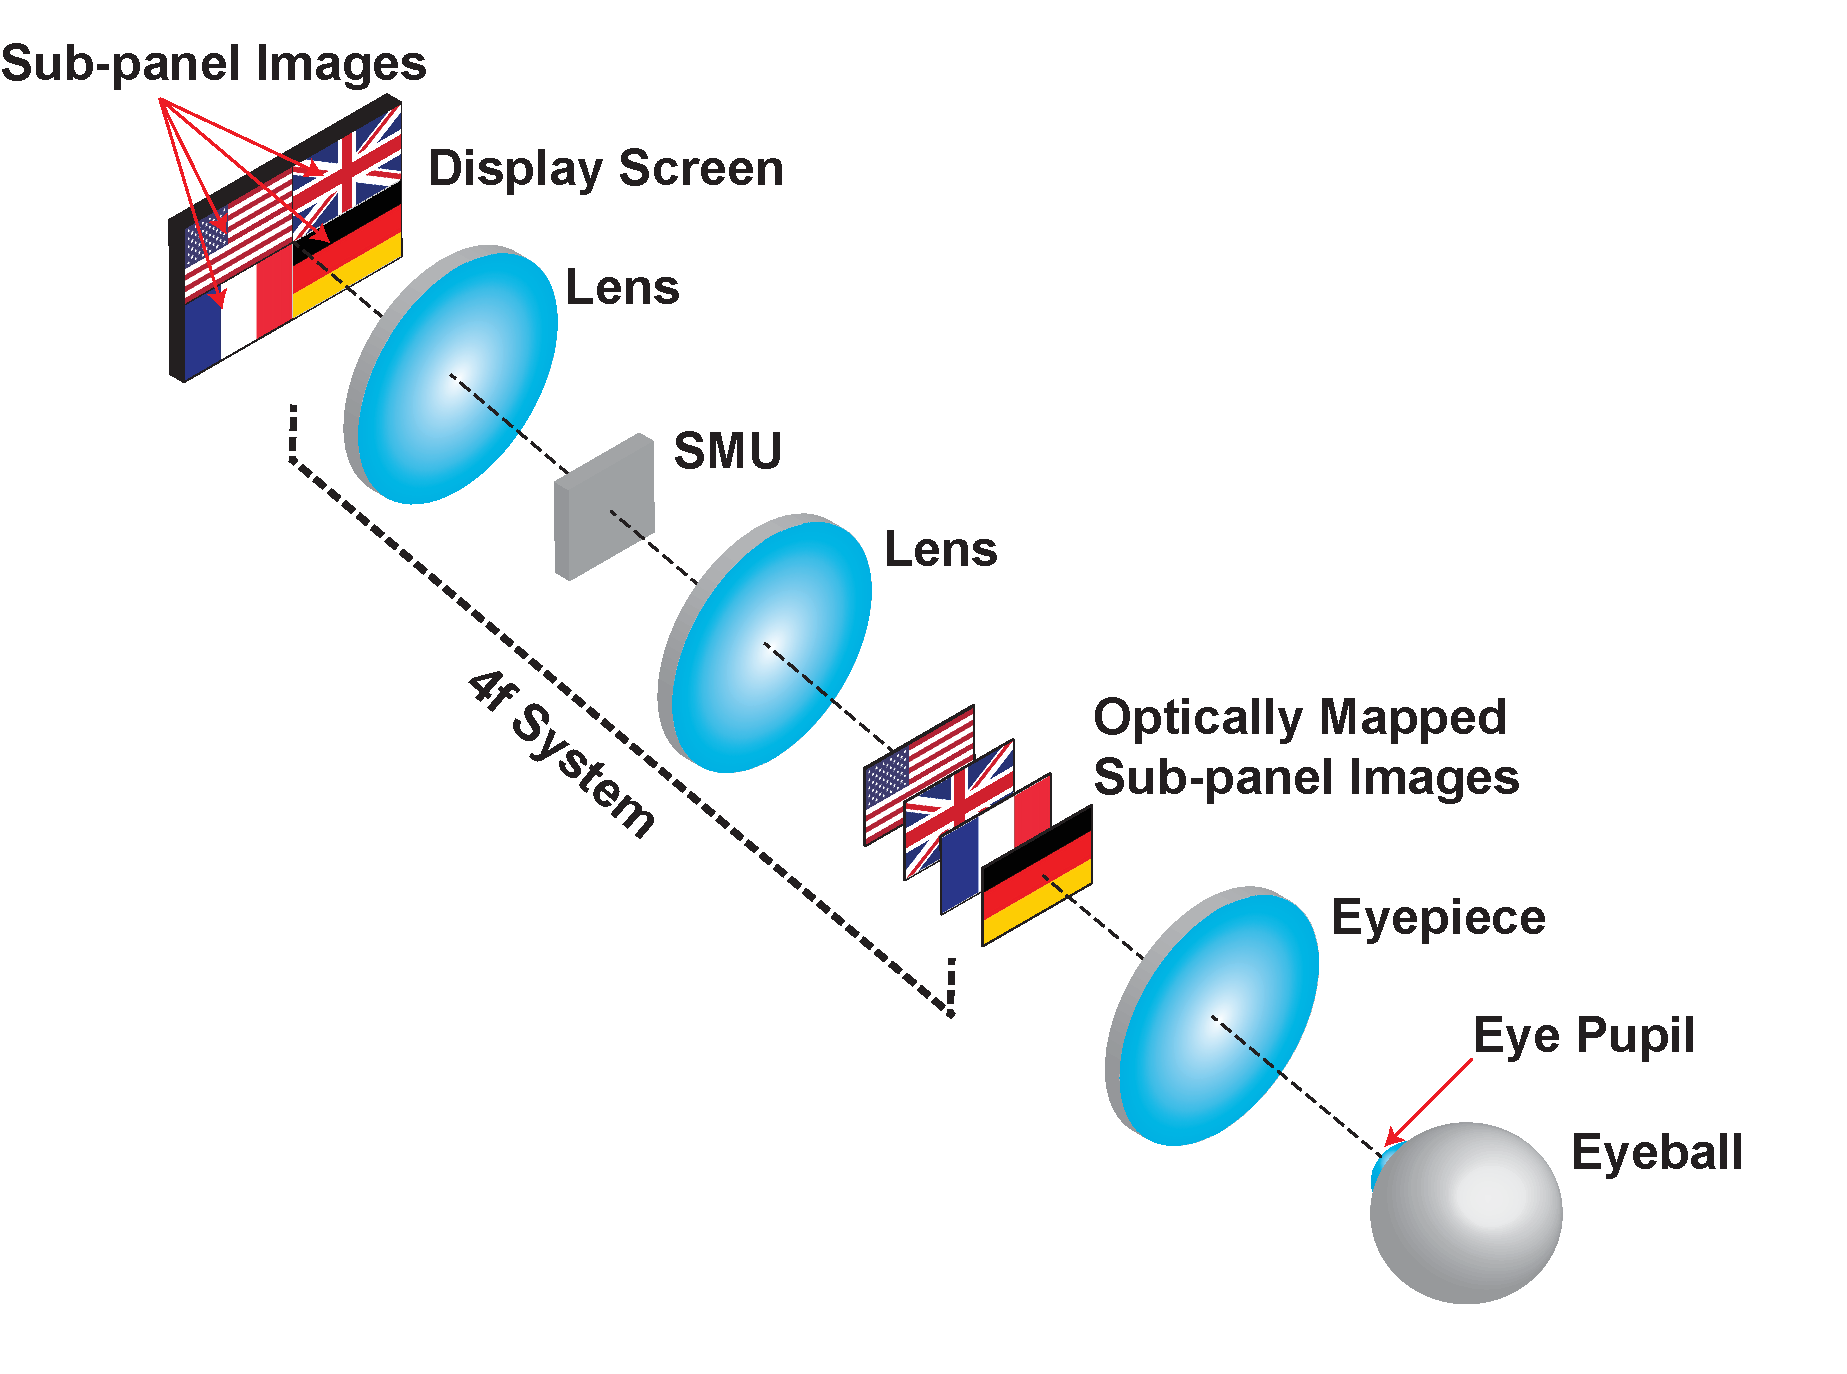
\includegraphics[width=\linewidth]{OMNIfig1}
\caption{Operating principle of the optical mapping near-eye 3D display (OMNI).}
\label{fig:1}
\end{figure}

To overcome above limitations, herein we present an optical mapping near-eye 3D display method (OMNI) which provides correct focus cues.  Based on a similar conceptual thread to the multi-plane display, our method maps different portions of a display screen to different depths while forcing their centers aligned. These intermediate depth images are then reimaged by an eyepiece and projected onto the viewer’s retina. The operating principle is shown in Fig. \ref{fig:1}.  A high-resolution 2D image is displayed at an electronic screen.  The image consists of several sub-panels, each targeting to be displayed at a designated depth. The workhorse of our system is a 4$f$ optical relay with a spatial multiplexing unit (SMU) located at the Fourier plane. The SMU functions as a multifocal off-axis Fresnel lens, adding both quadratic and linear phase terms to the incident wavefront. The quadratic phase terms axially shift sub-panel images to designated depths, while the linear phase terms laterally shift the centers of sub-panel images to the optical axis. As a result, the sub-panel images are axially mapped to different locations but laterally aligned at the output end, forming a discrete light field.  Finally, these intermediate depth images are collected by an eyepiece and enter the eye pupil. Depending on their relative axial positions, the viewer perceives these multi-depth images at a distance from near eye to infinity. It is worthy nothing that, unlike the previous spatial multiplexing approach \cite{hoffman2008vergence}, our system requires only one display screen at the input, thereby maintaining a compact form factor and low power consumption.

As the core component, the SMU can be either reflective or transmissive. In our system, we adopted a reflective configuration and employed a liquid-crystal-on-silicon (LCOS) spatial light modulator (SLM) as the SMU. The optical setup is illustrated in Fig. \ref{fig:2}. The light emanated from a monochromatic organic light emitting diode (OLED) screen (MDP02BCYM, Microoled) is filtered both in color (central wavelength, 550 nm; bandwidth, 10 nm) and polarization. The filtered light then passes through a 50:50 beam splitter, followed by being collimated by an infinity-corrected microscope objective (2X M Plan APO, Edmund Optics). We placed the LCOS-SLM at the exit pupil of the objective lens to modulate the phase of the incident light. The reflected light is collected by the same objective lens, reflected at the beam splitter, and forms intermediate images at varied depths in front of an eyepiece (focal length, 25 mm).

\begin{figure}[htbp]
	\centering
	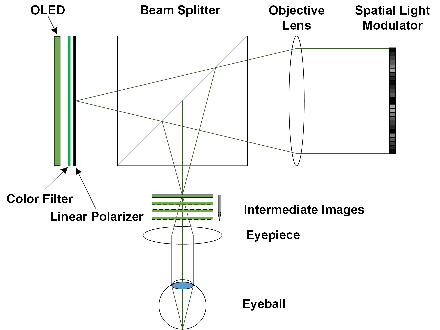
\includegraphics[width=\linewidth]{OMNIfig2}
	\caption{Schematic of OMNI display based on spatial-multiplexing multiplane display using a spatial light modulator.}
	\label{fig:2}
\end{figure}

To map sub-panel images to the designated locations, ideally, we need to display a phase pattern on the LCOS-SLM in the form:
\begin{equation}
\varphi(x,y) = \sum_{i}[ \frac{\pi (x^{2}+y^{2})}{\lambda f_{i}} + \frac{2 \pi}{\lambda}(\sin \frac{l_{x_i}}{2f_{o}}x +\sin\frac{l_{y_i}}{2f_{o}}y)],
\label{eq:1}
\end{equation}
where $\lambda$ is the light wavelength, $f_i$ is the effective focal length that adds optical power to the sub-panel image $i$ that is mapped at designated dioptric depth, $f_o$ is the focal length the objective lens, $l_{x_i}$ and $l_{y_i}$ are center coordinates of sub-panel image $i$ at the OLED.  Because each sub-panel image requires different $f_i$, $l_{x_i}$, and $l_{y_i}$, we sum phase terms over all indices, yielding a multiplexed phase pattern which acts as a multifocal off-axis lens. However, in practice, the LCOS-SLM can only address 8-bits phase levels (gray level patterns)   and the displayed wrapped phase is restrained within [0,2$\pi$]. To generate a phase pattern that is mathematically equivalent to $\varphi (x,y)$, we adopted an optimization algorithm, weighted Gerchberg-Saxton (GSW) \cite{di2007computer}. GSW starts with an initial guess for the phase $\varphi _{i}$ designated for each sub-panel image $i$ and employs adaptive weights \cite{bianchi2010real} that are adjusted accordingly after each cycle to make the outcome approach the ideal phase pattern. Within cycles of iterations, the converged results yield the optimized phase pattern.
  
In addition, to create a 3D scene with continuous depth perception, we employed a depth-weighted blending algorithm \cite{ravikumar2011creating} to produce the content of sub-panel images at the input display screen.  An intuitive linear depth-weighted blending algorithm was applied, in which the image intensity at each depth plane is proportional to the dioptric distance of the point from that plane along a line of sight. Then the sum of the intensities of all the focal planes will remain constant for all the dioptric depth, thus guarantee a continuous 3D scene without visible discontinuities between adjacent focal planes.

The output 3D images share the same dynamic range and the image refresh rate of the display screen, which can reach 12 bits and 30 Hz. Since there are four sub-panel images that correspond the depth planes, the spatial resolution of our system is ¼ of the size of the display screen. In the ideal scenario, the display pixels will be the multiplication of the number of depth planes and the spatial resolution. Thus the pixel size of the 3D image will be around $1000\times1000$, with the image size of about $5\times5$ mm$^2$. Dependent on the focal length of the eyepiece (25 mm), the field of view is around 10 degrees, which can be further extended using eyepiece with shorter focal length.

The OMNI display offers a prominent advantage in adaptability. Because the sub-panel images occupy the same display screen at the input end, the product of a depth plane’s lateral resolution ($L\times M$ pixels) and the number of depth planes ($N$) must not be greater than the total number of pixels ($P$) at the display screen, \textit{i.e.},  $L\times M\times N\leq P$. Taking this constraint into consideration, we can configure the system working in two modes which selectively bias the lateral resolution and the depth plane spacing, respectively, simply by changing the phase patterns on the LCOS-SLM. For the given high-resolution OLED ( $P$ = 4 megapixels) and a depth range of three diopters, we summarize two typical display settings in Table \ref{table:1}. The scalability of display parameters thus grants us more freedom to adapt the OMNI display to the depicted scene at a single frame level. 

Furthermore  , unlike temporal-multiplexing-based multi-plane display \cite{hu2014design}, herein the image frame rate and dynamic range are decoupled from the number of depth planes and thereby limited by only the display screen itself. Using the given OLED, we can display a high dynamic range (12 bits) 3D video in real time (30 Hz).

\begin{table}[htbp]
\centering
\caption{System parameters of an OMNI display.}
\label{table:1}
\begin{tabular}{p{3.5cm}p{2cm}p{2cm}}
	\hline
	&Lateral resolution (pixels)&Depth plane spacing (D)\\
	\hline
	High lateral resolution mode&1000$\times$1000&1D\\
	Dense depth sampling mode&500$\times$500&0.2D\\
	\hline
\end{tabular}
\end{table}

To visualize the intermediate depth images, we performed a simple mapping experiment. At the input end, we displayed four letters “U”, “I”, “U”, “C” in the four sub-panels of OLED (Fig. \ref{fig:3}(a)). We placed a camera at the focus of the eyepiece, translated it towards the eyepiece, and captured images at four nominal depth planes (0D, 1D, 2D, and 3D).  The remapped letter images at these four depths are shown in Fig. \ref{fig:3}(b)-(e), respectively. As expected, the letters appear sharp at their designated depths while blurred elsewhere. 

\begin{figure}[htbp]
\centering
\includegraphics[width=\linewidth]{OMNIfig3}
\caption{(a)Schematic of the mapping experiment and (b) through (e) the resultant intermediate images of “UIUC” letter pattern, showing on-focus letter “U,” “I,” “U,” “C” respectively from far-end to near-end towards the eyepiece.}
\label{fig:3}
\end{figure}

Next, we varied the depth plane spacing and accommodation distance to evaluate their effects on the image contrast.  In Experiment I, we placed a camera in front of the eyepiece to mimic an eye that focused at 1.5D. We displayed two sub-panel images at the OLED and projected them to (1.5+$\frac{\Delta z}{2}$)D and (1.5-$\frac{\Delta z}{2}$)D, respectively. We varied the depth plane spacing, $\Delta z$, through changing the effective focal length $f_i$ in the phase pattern at LCOS-SLM (Eq. \ref{eq:1}).  Accordingly, we acquired the depth-fused images at the camera, and calculated the image modulation contrast using the slanted edge method \cite{hu2014design}.  The dependence of modulation contrast on the depth plane spacing $\Delta z$ is shown in Fig. \ref{fig:4}(a). In general, the modulation contrast degrades as the depth plane spacing increases. However, for a given number of depth planes, decreasing the depth plane spacing will unfavorably reduce the total depth range. Therefore, one must balance the image quality for a desired depth range.

\begin{figure}[htbp]
	\centering
	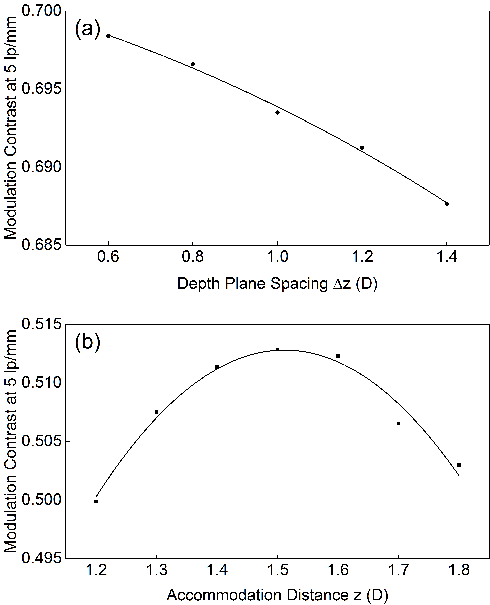
\includegraphics[width=\linewidth]{OMNIfig4}
	\caption{(a) Data points and the fitted curve at the same spatial frequency (5 lp/mm) of each MTF curves in the depth-fused dual-focal-plane display as a function of the plane spacing $\Delta$z. (b)Same data points and the fitted curves as a function of the focus depth z.}
	\label{fig:4}
\end{figure} 

In Experiment II, we varied the focal depth, z, of the camera to mimic the accommodation distance change of the eye. At the input end, we rendered the sub-panel image contents with a weighted dioptric distance centered at the dioptric midpoint of the two depth planes, 1.5D, and set the depth plane spacing $\Delta z$ to 1D.  We captured images at a variety of dioptric accommodation distance z, and derived the correspondent image modulation contrasts.  As expected, the result (Fig. \ref{fig:4}(b)) shows that the modulation contrast reaches the maximum at z = 1.5D, and degraded smoothly around this depth. This indicates that we get a correct focus cues around the weighted dioptric depth, which is particularly important for applications where most displayed objects locate around a given depth. By producing the contents with a central weight at this depth, we can accordingly optimize the system imaging performance.

\begin{figure}[htbp]
\centering
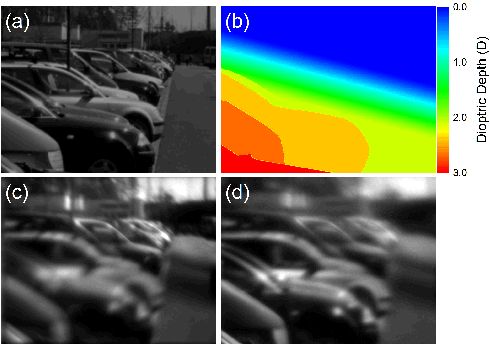
\includegraphics[width=\linewidth]{OMNIfig5}
\caption{(a) The reference all in focus 2D image and (b) the depth map of the scene.  Depth-fused images captured at (a) the far-end (0D) and (b) the near-end (3D). }
\label{fig:5}
\end{figure}

Last, we tested our system by displaying a complex 3D scene.  The reference all-in-focus image and the corresponding depth map are shown in Fig. \ref{fig:5}(a) and (b), respectively.  We generated the display contents at four nominal depth planes with $\Delta z$ = 1D and weighted against a central depth at 1.5D.  Again, we varied the focal depth the camera to mimic the accommodation distance change of the eye. The depth-fused images captured at 0D and 3D are shown in Fig. \ref{fig:5}(c) and (d), respectively, consistent with the depth map (Fig. \ref{fig:5}(b)). The resultant focus cues therefore match with those provided by binocular stereopsis. 

In the presented system, we chose a LCOS-SLM as the SMU to accomplish the optical mapping. Although not demonstrated,  the SMU can also be other phase modulation devices, such as a volume holography grating \cite{sinha2004imaging}\cite{luo2010simulations} or a distorted phase grating \cite{dalgarno2010multiplane}\cite{blanchard1999simultaneous}. Similar to the LCOS-SLM, both these phase modulators can function as a multifocal off-axis Fresnel lens, directing the sub-panel images to the designated depths while forcing their centers aligned.   However, unlike the LCOS-SLM, the volume holograph grating and distorted phase grating are passive devices, a fact that leads to both pros and cons. On the one hand, passive phase modulators require no power supplies, reducing the system volume as well as the power consumption. On the other hand, because their phase patterns are fixed, passive phase modulators cannot scale the display parameters in the adaptive fashion as previously discussed.

Although herein we demonstrated only monochromatic display mode, the OMNI display is capable of color reproduction. Using a white light OLED as the input screen, we can further split a sub-panel image into three channels, followed by covering them with a red, green, and blue color filter, respectively. Accordingly, at the LCOS-SLM, we must display a phase pattern that compensates for the wavelength difference, thereby mapping these filtered images to the same depth. Nevertheless, given a desired depth plane spacing, introducing colors will unfavorably reduce the lateral resolution by a factor of three.

In summary, we developed a novel optical mapping method for near-eye 3D display (OMNI) with correct focus cues that are consistent with binocular vision, thus eliminating the vergence-accommodation conflict. Through mapping different sub-panel images of a display screen to different axial depths, we can create a high-resolution 3D image over a depth range from 3 dipters to infinity. The image dynamic range and refresh rate are limited by only the display screen itself and can reach up to 12 bits and 30 Hz, respectively. Moreover, our system features a compact form factor and low power consumption thanks to a single display screen in use.  In sight of advantages above, we envision the optical mapping method will lead to a new generation of 3D display and exhibit great potentials for various wearable display applications.\\

\textbf{Funding.} This work was supported in part by NSF CAREER grant (xx) and discretionary funds from UIUC.\\

\textbf{Acknowledgments.} The authors thank Nuochen Lyu and Minkang Yang for their helpful discussions in the depth-weighted blending and the optimization algorithm.

% Bibliography
\bibliography{OMNI}

% Full bibliography added automatically for Optics Letters submissions
% Note that this extra page will not count against page length
\ifthenelse{\equal{\journalref}{ol}}{%
\clearpage
\bibliographyfullrefs{OMNI}
}{}
 
\end{document}
